\documentclass{IEEEcsmag}

\usepackage[colorlinks,urlcolor=blue,linkcolor=blue,citecolor=blue]{hyperref}
\expandafter\def\expandafter\UrlBreaks\expandafter{\UrlBreaks\do\/\do\*\do\-\do\~\do\'\do\"\do\-}
\usepackage{upmath,color}

\usepackage[spanish]{babel}
%\usepackage[latin1]{inputenc}
\usepackage[utf8]{inputenc}  

\jvol{1}
\jnum{1}
\paper{1}
\jmonth{Noviembre}
\jname{ITICs letters}
\jtitle{Proyectos Integradores}
\pubyear{2023}
\usepackage{cite}
\usepackage{amsmath,amssymb,amsfonts}
\usepackage{algorithmic}
\usepackage{graphicx}
\usepackage{textcomp}
\usepackage{xcolor}
\usepackage{listings}

\newtheorem{theorem}{Theorem}
\newtheorem{lemma}{Lemma}



\setcounter{secnumdepth}{0}

\begin{document}

%imprimir código
\lstnewenvironment{javaCode}[1][]
{\lstset{
    language=Java,
    basicstyle=\scriptsize\ttfamily,
    numbers=none, % Modificado: quitar los números de línea
    keywordstyle=\color{blue},
    commentstyle=\color{gray},
    stringstyle=\color{purple},
    breaklines=true,
    breakatwhitespace=true,
    tabsize=4,
    showspaces=false,
    showstringspaces=false,
    frame=single,
    captionpos=b,
    floatplacement=!h,
    #1
}}
{}


\sptitle{Proyecto Integrador de Primer Semestre}

\title{Software de resolución de problemas de Ingeniería }

\author{Cuadros Romero Francisco Javier}
\affil{Instituto Tecnológico Superior del Occidente del Estado de Hidalgo, Mixquiahuala, Hgo., 42700, Mexico}

\author{Neri Pérez Giovany Humberto}
\affil{Instituto Tecnológico Superior del Occidente del Estado de Hidalgo, Mixquiahuala, Hgo., 42700, Mexico}

%\author{Third Author III}
%\affil{Institute, City, (State), Postal Code, Country}

\markboth{ITSOEH/ITICS/PROYECTO INTEGRADOR PRIMER SEMESTRE}{THEME/FEATURE/DEPARTMENT}

\begin{abstract}
Un resumen (abstract) es un párrafo único que resume los aspectos importantes del manuscrito. A menudo indica si el manuscrito es un informe de un trabajo nuevo, una revisión o una descripción general, o una combinación de ambos. No cite referencias en el resumen. Este tipo de documento debe incluir contenido propiedad de los autores; es decir, no debe contener contenido de otras fuentes, ademas la redacción debe  estar dirigida a un tipo de lector técnico general. Este archivo se encuentra disponible en \href{https://github.com/fcuadrosgithub/integrador-primero.git}{https://github.com/fcuadrosgithub/integrador-primero.git}.
\end{abstract}

\maketitle
\chapteri{L}a introducción debe proporcionar información general (incluidas referencias relevantes) y debe indicar el propósito del manuscrito. En esta sección describa de manera clara y precisa el objetivo del proyecto integrador, la metodología que piensa usar y los resultados obtenidos de manera muy general. Dentro de esta sección puede citar trabajos relevantes de otros si lo cree necesario.

Esta sección debe dar un panorama muy general al lector de cual es el problema a resolver, que metodología utilizó para dar solución al problema y cuales fueron los resultados obtenidos. 

La redacción del manuscrito debe ser en tercera persona y queda estrictamente prohibido el uso de palabras coloquiales o Español informal. En lugar de esto utilice un lenguaje formal que el mayor numero de personas pueda entender.

\section{COPYRIGHT Y ACCESO ABIERTO}

Una vez que los autores entreguen este documento para su evaluación también seden los derechos del contenido de este manuscrito a la carrera de Ingeniería en Tecnológicas de la Información y Comunicaciones (ITICs) del Instituto Tecnológico Superior del Occidente del Estado de Hidalgo (ITSOEH). Esto conlleva que la carrera puede usar el contenido de este articulo para efectos de difusión del quehacer de los estudiantes de la carrera o en cualquier otra actividad que la carrera considere pertinente. Cabe mencionar que en ningún momento el orden o los nombres de los autores sera modificado de ninguna manera y siempre se les dará el crédito correspondiente. 
\section{PROBLEMAS}
A continuación se describen los problemas que el equipo deberá resolver.
\begin{enumerate}
\item Dados 2 puntos $A \mbox{ y } B$ con coordenadas $x_{1}, y_{1}$ y $x_{2}, y_{2}$  respectivamente. Regresar la ecuación de la recta y el ángulo interno $\alpha$ que se forma entre el eje horizontal y la recta. 
%Por ejemplo con los puntos $A(2, 1)$ y $B(-3, 2)$ la ecuación debe ser $y = -\frac{1}{5}x + \frac{7}{5}$. 
\item Dada una ecuación cuadratica regresar los valores de las raíces en caso de que estén sobre el conjunto de los números reales, en caso contrario indicar que la solución esta en el conjunto de los números complejos. 
\item Dada una circunferencia con centro en el punto $C$ con coordenadas $(x_{1}, y_{1})$ y radio $r$, evaluar si un punto $T$ con coordenadas $(x_{2}, y_{2})$ esta dentro del area de la circunferencia.
\item Dado un numero decimal entero positivo o negativo regresar su equivalente en binario.
\item Dado un numero binario de $n$ bits regresar su equivalente en decimal.
\item Dada una tabla de verdad de $n$ bits generar la expresión booleana que genere de manera fidedigna las salidas de esta tabla.
\end{enumerate}





% ⚠️⚠️⚠️⚠️⚠️⚠️⚠️⚠️⚠️ PROBLEMA 1 ⚠️⚠️⚠️⚠️⚠️⚠️⚠️⚠️⚠️
\section{Sección Problema 1}
\newpage
Contenido del primer problema...
\newpage
Contenido del primer problema...





% ⚠️⚠️⚠️⚠️⚠️⚠️⚠️⚠️⚠️ PROBLEMA 2 ⚠️⚠️⚠️⚠️⚠️⚠️⚠️⚠️⚠️
\section{Sección Problema 2}

\section*{Introducción}
Este proyecto aborda el problema de resolver ecuaciones cuadráticas, identificando si sus raíces son reales o complejas. La resolución de ecuaciones cuadráticas es una tarea fundamental en álgebra y tiene aplicaciones en diversos campos, desde física hasta ingeniería.

\section*{Descripción del problema:}
Se debe determinar si las raíces de una ecuación cuadrática son reales o complejas. Si son reales, se calculan y se proporcionan los valores. Si son complejas, se indica que la solución está en el conjunto de los números complejos.


\section*{Definición de solución:}
Para determinar la naturaleza de las raíces de una ecuación cuadrática de la forma  (\(ax^2 + bx + c = 0\)), se evalua el discriminante. Si es negativo, las raíces son complejas. De lo contrario, se calculan utilizando la fórmula cuadrática estándar:

\[ x = \frac{-b \pm \sqrt{b^2 - 4ac}}{2a} \]

Donde:
\begin{itemize}
    \item \(a\), \(b\), y \(c\) son los coeficientes de la ecuación cuadrática.
    \item El valor del discriminante determina si las raíces son reales o complejas y proporciona información sobre la cantidad de raíces distintas.
\end{itemize}



\begin{figure}[h!]
    \centering
    \includegraphics[width = 6 cm]{imagen/prob2.jpg}
    \caption{Gráfica de la ecuación de la solución de raíces}
    \label{fig:GraficaEcuacionRecta}
\end{figure}

\section*{Diseño de la solución:}

Para el diseño de la solucion se seguiran los siguientes pasos:
\begin{itemize}
    \item Calcular la pendiente de la recta.
    \item Calcular la ordenada en el origen de la recta.
    \item Determinar el ángulo interno
    \item Devolver la ecuación de la recta y el ángulo
\end{itemize}

Tal y como se muestraen el siguientediagrama de flujo.

\begin{figure}[h!]
    \centering
    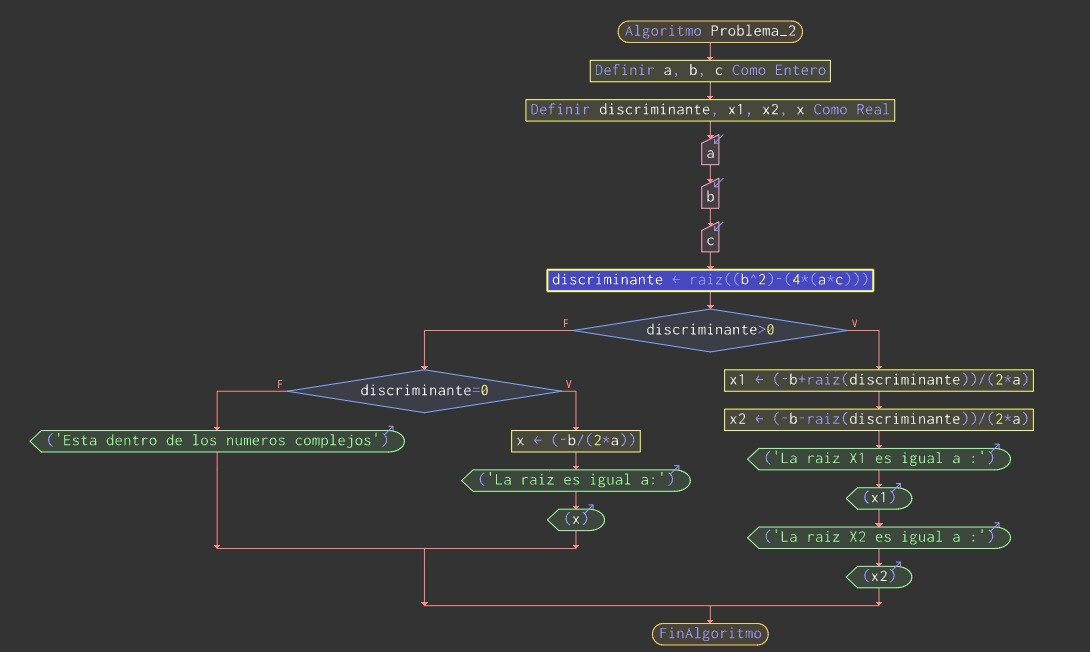
\includegraphics[width = 6 cm]{imagen/a.jpeg}
    \caption{Gráfica de la ecuación de la solución de raíces}
    \label{fig:GraficaEcuacionRecta}
\end{figure}

\section*{Desarrollo de la solución:}
La implementación del código solicita al usuario los coeficientes \(a\), \(b\), y \(c\), calcula el discriminante y aplica la lógica mencionada para determinar la naturaleza de las raíces. 
\begin{javaCode}
 Scanner in= new Scanner(System.in);
        //Solicitar los datos para la formula general.
        
        System.out.println("""
                           "Ingresa los puntos a, b, c.
                           Separadas por una coma(a, b, c): 
                           """);
        String [] datos=in.nextLine().split(",");
        //cerrar el escaneo
        in.close();
        
\end{javaCode}
\newpage
Posteriormente se convierten los valores de los puntos A, B, C. en valores enteros para ser utilizados  en la formula general .

\begin{javaCode}
    //Asigna Valores de a, b, c en enteros.
        int a= Integer.parseInt(datos[0].trim());
        int b= Integer.parseInt(datos[1].trim());
        int c= Integer.parseInt(datos[2].trim());
        
\end{javaCode}
Una vez normalizados los datos, se calcula la discriminante.
\begin{javaCode}
    //Calcula la discriminante
    double discriminante=(Math.pow(b, 2)-(4*(a*c)));
\end{javaCode}

Ya que tenemos el resultado de la discriminante, dependiendo de este se realizara la operación justa, o se dirá que la discriminante esta dentro de los números complejos.\\
Si la discriminante es mayor que cero se realiza la siguiente operación y se imprimen en pantalla los 2 posibles resultados.:
\begin{javaCode}
    if (discriminante>0) {
            double x1=(-b+Math.sqrt(discriminante))/(2*a);
            
            double x2=(-b-Math.sqrt(discriminante))/(2*a);
            System.out.println("La raiz x1 es igual a " + x1);
            System.out.println("La raiz x1 es igual a " + x2);
            
        }
\end{javaCode}
En caso de que la discriminante sea igual a cero se realiza el siguiente calculo y se imprime el resultado en pantalla.:
\begin{javaCode}
    else if(discriminante==0){
            double x=(-b/(2*a));
            System.out.println("La raiz es igual a " + x);
        }
\end{javaCode}
Por ultimo, si la discriminante es menor a cero solo se imprimira en pantalla:\\"Esta dentro de los numeros complejos"
\begin{javaCode}
    else{
            System.out.println("Esta dentro de los numeros complejos");
        }
\end{javaCode}

\section*{Depuración y pruebas:}
\begin{center}
\begin{tabular}{|c|c|c|c|}
\hline
\textbf{\(a\)} & \textbf{\(b\)} & \textbf{\(c\)} & \textbf{\(Resultado\)} \\
\hline
1 & -3 & 2 & Raíces reales: \(x_1 = 2, x_2 = 1\) \\
\hline
1 & 2 & 1 & Raíz real única: \(x = -1\) \\
\hline
1 & -2 & 5 & Raíces complejas \\
\hline
\end{tabular}
\end{center}

\section*{Conclusión}
En resumen, el programa aborda la resolución de ecuaciones cuadráticas, clasificando las raíces entre reales y complejas mediante la evaluación del discriminante, destacando la utilidad de la fórmula cuadrática en este contexto.
\newpage





% ⚠️⚠️⚠️⚠️⚠️⚠️⚠️⚠️⚠️ PROBLEMA 3 ⚠️⚠️⚠️⚠️⚠️⚠️⚠️⚠️⚠️
\section{Sección Problema 3}
%Lizbeth

\section*{Descripción del problema:}
\begin{enumerate}
El problema 3 busca evaluar si un punto $T$ con coordenadas $(x_{2}, y_{2})$ esta dentro del área de la circunferencia, sabiendo que el punto $C$ se encuentra en el centro de la misma. Lo cual solo el usuario ingresara las coordenadas $(x_{1}, y_{1})$ y $(x_{2}, y_{2})$  y el radio $r$ para realizar el proceso de la  ecuación que se ocupo, y presentar la respuesta.
\end{enumerate}


\section*{Definición de solución:}
La solución para evaluar si un punto $T$ con coordenadas $(x_{2}, y_{2})$ está dentro del área de una circunferencia con centro en el punto $C$ con coordenadas $(x_{1}, y_{1})$ y radio $r$ implica utilizar la fórmula de la distancia euclidiana, la distancia se calcula como la raíz cuadrada de la suma de los cuadrados de las diferencias entre las coordenadas x y las coordenadas y de ambos puntos:
distancia = 
\begin{equation}
   \sqrt{ (x_2 - x_1)^2 + (y_2 - y_1)^2 }     
\end{equation}



Al final solo comparamos la distancia calculada con el radio $r$ de la circunferencia:
\begin{enumerate}
\item Si la distancia es mayor que el radio $r$, el punto $T$ está fuera de la circunferencia.
\item Si la distancia es igual al radio $r$, el punto $T$ está en el borde de la circunferencia.
\item Si la distancia es menor que el radio $r$, el punto $T$ está dentro del área de la circunferencia.    
\end{enumerate}


\section*{Diseño de la solución:}
\begin{enumerate} 
\item Solicitar al usuario que ingrese las coordenadas del punto $C$ y el punto $T$, es decir $(x_{1}, y_{1})$ y $(x_{2}, y_{2})$ y el radio $r$.
\item Calcular la distancia entre el centro y el punto.
\item Verificar si el punto está dentro del área de la circunferencia
\item Al final mostrar el resultado al usuario 
\end{enumerate}


\section*{Desarrollo de la solución:}
El algoritmo de solución del problema 3 comienza utilizando un objeto Scanner para leer las coordenadas del centro (punto $C$), el radio $r$ y las coordenadas del punto a verificar (punto $T$) desde la entrada estándar. Las coordenadas se ingresan en el formato $"x, y"$ separadas por una coma.
\begin{javaCode}
Scanner datC = new Scanner(System.in);
        System.out.print("""
                         Ingrese las coordenadas del punto C 
                         seperadas por una coma (x1, y1):
                         """);
    String[] puntoC = (datC.nextLine()).split(",");
        
    System.out.print("Ingrese el radio de la circunferencia: ");
    float r = datC.nextFloat();
    datC.nextLine();
    
    System.out.print("""
                         Ingrese las coordenadas del punto T
                         seperadas por una coma (x2, y2): 
                         """);
    String[] puntoT = (datC.nextLine()).split(",");
    datC.close();
\end{javaCode}
Posteriormente se convierten los valores de los puntos $(x_{1}, y_{1})$ y $(x_{2}, y_{2})$. en valores enteros para ser utilizados  en la ecuación de la distancia:

\begin{javacode}
    int x1 = Integer.parseInt(puntoC[0].trim());
    int y1 = Integer.parseInt(puntoC[1].trim());
        
    int x2 = Integer.parseInt(puntoT[0].trim());
    int y2 = Integer.parseInt(puntoT[1].trim()); 
\end{javacode}
Después el valor de las coordenadas del punto $C$ y del punto $T$ se convierten a números enteros y se calcula la distancia entre ellos utilizando la fórmula de la distancia euclidiana.
\begin{javacode}
float distancia = (float)Math.sqrt(Math.pow(x2 - x1, 2) + Math.pow(y2 - y1, 2)); 
\end{javacode}

Al final se verifica la ubicación del punto, se comparan la distancia calculada con el radio $r$ de la circunferencia para determinar la ubicación del punto $T$. 
Dependiendo de la comparación, se imprime un mensaje indicando si el punto está dentro de la circunferencia, en el borde o fuera de ella.
\begin{javacode}
if (distancia > r) {
     System.out.println("El punto T("+x2+","+y2+") esta fuera de la circunferencia");
     }else if (distancia == r) {
     System.out.println("El punto T("+x2+","+y2+") esta en la circunferencia");
    }else{
     System.out.println("El punto T("+x2+","+y2+") esta dentro de la circunferencia");
    }
\end{javacode}


\section*{Depuración y pruebas:}
\begin{table}[h!]
     \centering
     \caption{Tabla de Corridas del problema 3}\\

     \begin{tabular}{|c|c|c|c|c|c|}
     \hline
    Corrida & Coordenadas $(x_{1}, y_{1})$& Coordenadas $(x_{2}, y_{2})$  &  Radio $r$ & Resultado\\
    \hline
    1  &  $(3,4)$ & $(9,2)$ & 10 & El punto $T$ esta adentro \\
    \hline
    2  &  $(5,2)$ & $(8,1)$ & 12 & El punto $T$ esta adentro \\
    \hline
    3  &  $(34,23)$ & $(-90,35)$ & 67 & El punto $T$ esta afuera \\
    \hline
    4  &  $(-27,3)$ & $(34,-5)$ & 30 & El punto $T$ esta afuera \\
    \hline
    5 &  $(2,8)$ & $(4,9)$ & 17 & El punto $T$ esta adentro \\
    \hline
     \end{tabular}
     \label{tab:my_label}
 \end{table}





% ⚠️⚠️⚠️⚠️⚠️⚠️⚠️⚠️⚠️ PROBLEMA 4 ⚠️⚠️⚠️⚠️⚠️⚠️⚠️⚠️⚠️
\section{Sección Problema 4}
\section*{Descripción del problema:}
Dado un numero decimal entero positivo o negativo regresar su equivalente en binario.
\newline

\section*{Definición de solución:}

El sistema de numeración decimal es un sistema posicional que utiliza la base diez para representar cantidades. En este sistema, se emplean diez dígitos distintos:
\newline

[ 0, 1 , 2, 3, 4, 5, 6, 7, 8, 9, 0 ] 
\newline


Mientras que el sistema binario, a diferencia del sistema decimal, se caracteriza por ser un sistema de numeración que utiliza solo dos dígitos, 0 y 1; Para representar información. Es la base fundamental de la computación digital y la electrónica digital, ya que los dispositivos electrónicos, como las computadoras, utilizan señales eléctricas que pueden estar en dos estados: encendido (representado por 1) o apagado (representado por 0).
\newline

Los términos "bit" (dígito binario) y "byte" (conjunto de 8 bits) son comunes en el contexto del sistema binario. La representación binaria es fundamental para entender cómo la información se almacena, procesa y transmite en sistemas digitales, incluyendo todas las computadoras y dispositivos electrónicos modernos.
\newline 

La conversión de un número decimal a binario se basa en el método de sucesivas divisiones por 2, que es una técnica fundamental en el sistema binario. Este proceso es especialmente aplicable a números naturales positivos. La esencia de la conversión radica en dividir repetidamente el número decimal por 2 y registrar los residuos en orden inverso al que fueron obtenidos.

\begin{figure} 
    \centering
    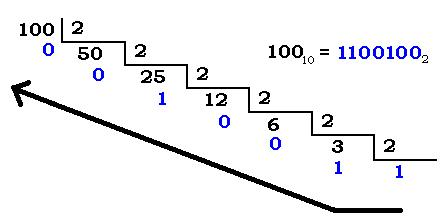
\includegraphics[width=0.6\linewidth]{conversion.jpg}
    \caption{Representación de la conversión}
    \label{fig: Conversion a Binario}
\end{figure}

Sin embargo, en el caso de números negativos, el proceso se complica y se introduce el concepto de complemento a 2, una técnica que implica obtener el complemento a 1 y sumar 1 al resultado para obtener la representación binaria del número negativo.La conversión a negativo tenemos 3 opciones 

\subsection{Complemento a 1:}
En el contexto del "complemento a 1" de un número binario, nos referimos a la secuencia de bits que se obtiene al invertir (cambiar de 0 a 1 y de 1 a 0) todos los bits del número original. Esta técnica es ampliamente utilizada en sistemas binarios para representar números negativos.
\newline

Por ejemplo, si tenemos el número binario 01010101, al aplicar el complemento a 1 obtendríamos 10101010, ya que hemos invertido cada bit. El complemento a 1 se utiliza principalmente para representar la magnitud negativa de un número binario y es una parte fundamental en el cálculo del complemento a 2."
\newline

\subsection{Complemento a 2:}
El proceso de obtener el complemento a 2 de un número binario es un paso esencial en la representación de números negativos en sistemas binarios. Este método se basa en la utilización del complemento a 1 y la adición de 1 al resultado
\newline


\section*{Desarrollo de la solución:}
El algoritmo de solución para la conversión 
Comienza solicitando al usuario un numero decimal entero ya sea este positivo o negativo .

\begin{javaCode}
    public static void main(String[] args) {
         // Crear variable de escaneo de datos
        Scanner decimal = new Scanner(System.in);

        // Solicitud del número decimal
        System.out.print("Ingrese el número decimal entero positivo o negativo: ");
        long numeroDecimal = decimal.nextLong();
\end{javaCode}

Posteriormente se agrega en el método principal, la instrucción para imprimir el resultado de la conversión, en caso de ser negativo se imprimen dos casos de complemento 1 y complemento 2.


\begin{javaCode}
    // Impresión del número convertido y su complemento
        System.out.println("El número convertido a binario es: " + decimalABinario(numeroDecimal));
        if (numeroDecimal < 0) {
            System.out.println("Complemento a 1: " + complementoAUno(numeroDecimal));
            System.out.println("Complemento a 2: " + complementoADos(numeroDecimal));
        }
\end{javaCode}

Después de obtener el número que se va a convertir, se procede a crear un método (decimalABinario) específico encargado de realizar la conversión a binario. Al ingresar a este método, el primer paso consiste en obtener el valor absoluto del número decimal.

\begin{javaCode}
  public static String decimalABinario(long decimal) {
        String binario = "";
        long numero = Math.abs(decimal); // Obtener el valor absoluto del número
\end{javaCode}


Ante posibles problemas se crean 2 casos,
Si el número es 0, retorna "0" directamente, ya que su representación en binario es igual.

\begin{javaCode}
    //Caso 1 ser igual a 0
    if (numero == 0) {
        return "0";
    }
\end{javaCode}

Si es diferente de 0, mediante un bucle, se procede a dividir de manera consecutiva el número decimal por 2, almacenando los residuos en la cadena binaria. Este proceso construye la representación binaria del número.

Ya no es necesario invertir la cadena ya que el residuo se concatena a la izquierda de la cadena.

\begin{javaCode}
    //Si es diferente de 0 
    while (numero != 0) {
        int residuo = numero % 2;
        //Concatenacion 
        binario = residuo + binario ; 
        numero = numero / 2;
    }
\end{javaCode}

Finalmente, en el caso de que el número decimal sea negativo, para el primer caso de complemento a 1, 

\begin{javaCode}
      if (decimal < 0) {
            // Complemento a 1
            binario = complementoAUno(decimal);
        }

    return binario;
\end{javaCode}

Aquí se define un método llamado complementoAUno que toma un número largo (long) como parámetro y devuelve una representación en forma de cadena del complemento a uno de ese número, aqui solo se invierten los bits.

\begin{javaCode}
        public static String complementoAUno(long numero) {
        StringBuilder complemento = new StringBuilder();
        String binario = Integer.toBinaryString(Math.abs((int) numero));

        // Invertir los bits
        for (char bit : binario.toCharArray()) {
            complemento.append(bit == '0' ? '1' : '0');
        }

        return "-" + complemento.toString();
    }


\end{javaCode}

Así mismo se hace otro método llamado (complementoADos), se toma un número, calcula su complemento a dos y devuelve la representación binaria de ese complemento con el signo negativo.

\begin{javaCode}
 public static String complementoADos(long numero) {
        int numeroPositivo = Math.abs((int) numero);
        String binarioPositivo = Integer.toBinaryString(numeroPositivo);
        StringBuilder bitsInvertidos = new StringBuilder();
\end{javaCode}

Se invierten los bits de una representación binaria almacenada en la cadena binarioPositivo. Utilizando un bucle for que itera sobre cada bit de la cadena. Dentro del bucle, la expresión bit == '0' ? '1' : '0' evalúa si el bit actual es '0'; en caso afirmativo, se agrega '1' al StringBuilder bitsInvertidos, de lo contrario, se agrega '0'. 

\begin{javaCode}
    // Invertir los bits
        for (char bit : binarioPositivo.toCharArray()) {
            bitsInvertidos.append(bit == '0' ? '1' : '0');
        }
\end{javaCode}

Este ultimo codigo lo que representa es el complemento 2, el cual al ya tener los bits invertidos solo suma 1 al, con Integer.parseInt(..., 2) automaticamente lo que hace java es pasarlo a base 2, solo cambia el signo y da el resultado.

\begin{javaCode}
    // Agregar 1 al resultado para obtener la representación de complemento a 2
        int resultado = Integer.parseInt(bitsInvertidos.toString(), 2) + 1;

        return "-" + Integer.toBinaryString(resultado);
    
\end{javaCode}
\subsection{Depuración}


\subsection{Pruebas de escritorio}
    Ejemplo 1: ( 9 8 5 2 ) \newline

\newline \begin{tabular}{|c|c|c|c|}
  \hline
  Dividendo & Divisor & Cociente & Residuo \\
  \hline
  9852 & 2 & 4926 & 0 \\
  4926 & 2 & 2463 & 0 \\
  2463 & 2 & 1231 & 1 \\
  1231 & 2 & 615 & 1 \\
  615 & 2 & 307 & 1 \\
  307 & 2 & 153 & 1 \\
  153 & 2 & 76 & 1 \\
  76 & 2 & 38 & 0 \\
  38 & 2 & 19 & 0 \\
  19 & 2 & 9 & 0 \\
  9 & 2 & 4 & 1 \\
  4 & 2 & 2 & 0 \\
  2 & 2 & 1 & 0 \\
  1 & 2 & 0 & 1 \\
  \hline
\end{tabular}
\newline 

Resultado: \(9852\) en binario es \( 10010001111100.\).
\newline


Ejemplo 2: ( 7 3 9) \newline  
\newline \begin{tabular}{|c|c|c|c|}
\hline
Dividendo & Divisor & Cociente & Residuo \\
\hline
739 & 2 & 369 & 1 \\
369 & 2 & 184 & 1 \\
184 & 2 & 92 & 0 \\
92 & 2 & 46 & 0 \\
46 & 2 & 23 & 0 \\
23 & 2 & 11 & 1 \\
11 & 2 & 5 & 1 \\
5 & 2 & 2 & 1 \\
2 & 2 & 1 & 0 \\
1 & 2 & 0 & 1 \\
\hline
\end{tabular}
\newline

Resultado: \(739\) en binario es \(1011100011.\).
\newline

Ejemplo 3: ( 3 7 4 )  \newline
\newline \begin{tabular}{|c|c|c|c|}
  \hline
  Dividendo & Divisor & Cociente & Residuo \\
  \hline
  374 & 2 & 187 & 0 \\
  187 & 2 & 93 & 1 \\
  93 & 2 & 46 & 1 \\
  46 & 2 & 23 & 0 \\
  23 & 2 & 11 & 1 \\
  11 & 2 & 5 & 1 \\
  5 & 2 & 2 & 1 \\
  2 & 2 & 1 & 0 \\
  1 & 2 & 0 & 1 \\
  \hline
\end{tabular}
\newline

Resultado: \(374\) en binario es \(101110110\).
\newline


Ejemplo 4: ( 3 4 2 1 ) \newline 
\newline \begin{tabular}{|c|c|c|c|}
  \hline
  Dividendo & Divisor & Cociente & Residuo \\
  \hline
  3421 & 2 & 1710 & 1 \\
  1710 & 2 & 855 & 0 \\
  855 & 2 & 427 & 1 \\
  427 & 2 & 213 & 1 \\
  213 & 2 & 106 & 1 \\
  106 & 2 & 53 & 0 \\
  53 & 2 & 26 & 1 \\
  26 & 2 & 13 & 0 \\
  13 & 2 & 6 & 1 \\
  6 & 2 & 3 & 0 \\
  3 & 2 & 1 & 1 \\
  1 & 2 & 0 & 1 \\
  \hline
\end{tabular}
\newline

Resultado: \(3421\) en binario es \( 110101100101.\).
\newpage





% ⚠️⚠️⚠️⚠️⚠️⚠️⚠️⚠️⚠️ PROBLEMA 5 ⚠️⚠️⚠️⚠️⚠️⚠️⚠️⚠️⚠️
\section{Sección Problema 5}
\section*{Descripción del problema:}
El reporte analiza el concepto de ingresar un número de tipo binario con $n$ bits, para posteriormente regresar su equivalente en decimal.

\section*{Definición de solución:}
Se planteó el generar un programa el cual sea capaz de realizar dicha premisa

\section*{Diseño de la solución:}
\begin{enumerate}
    \item Solicitar al usuario que ingrese el número binario de n bits.
    \item Validar que el número binario ingresado sea válido, es decir, que esté compuesto únicamente de 0's y 1's y tenga una longitud de n bits.
    \item Calcular el número decimal equivalente utilizando el método binAdecimal.
    \item Mostrar el resultado al usuario.
\end{enumerate}

\section*{Desarrollo de la solución:}
El algoritmo de solución del problema comienza solicitando al usuario teclee el número binario a convertir, para posteriormente almacenarlo en la variable $nbinario$:.
\begin{javaCode}
Scanner bin = new Scanner(System.in);
    System.out.println("Ingresa el numero binario: ");
    String nbinario = bin.nextLine();
    bin.close();
\end{javaCode}

Por consiguiente, se declara la variable donde se va a alacena1r el dato y el mensaje a imprimir en pantalla de la operación de conversión.

\begin{javaCode}
int num = binAdecimal(nbinario);
System.out.println("El numero decimal equivalente es: " + num);

\end{javaCode}

Como el procedimiento de conversión se realizó dentro de una clase privada, se creo una de estas para posteriormente hacer el procedimiento, aquí se declara la clase y se definen las variables con el tipo de dato que estas van a llegar a ser.

\begin{javaCode}
public static int binAdecimal(String binario){
    int n = binario.length();
    int decimal = 0;
    }
\end{javaCode}

Luego de haber definido todas nuestras variables, viene el procedimiento de resolución del programa, Para convertir un número binario a decimal, podemos utilizar un bucle "$for$". Primero, inicializamos una variable 'decimal' en 0. Luego, recorremos cada dígito del número binario utilizando la variable $i$ como contador.

\begin{javaCode}
    for (int i = 0; i < n; i++) {
    }
\end{javaCode}

En cada iteración del bucle, extraemos el dígito binario correspondiente utilizando la función "$Character.getNumericValue(binario.charAt(i))$". Este paso convierte el carácter binario en un entero.

\begin{javaCode}
    int bit=Character.getNumericValue
        (binario.charAt(i));
\end{javaCode}

Luego, multiplicamos este dígito por 2 elevado a la potencia correspondiente. Utilizamos la fórmula "$bit * Math.pow(2, n - 1 - i)$" para realizar esta multiplicación, donde "$bit$" es el dígito binario, $n$ es el tamaño del número binario y "$i$" es el contador del bucle.

\begin{javaCode}
decimal += bit * Math.pow(2, n - 1 - i);
\end{javaCode}

Finalmente, sumamos el resultado de cada multiplicación a la variable $decimal$.
Al finalizar el bucle, la variable $decimal$ contendrá el valor decimal equivalente al número binario original.

El código queda de la siguiente manera:
\begin{javaCode}
    for (int i = 0; i < n; i++) {
    int bit = Character.getNumericValue
    (binario.charAt(i));
    decimal += bit * Math.pow
    (2, n - 1 - i);
    }
\end{javaCode}

\section*{Depuración y pruebas:}
 
 \begin{table}[h]
     \centering
     \caption{Tabla de Corridas}
     
     \begin{tabular}{|c|c|c|}
     \hline
        Corrida & Binario & Decimal\\
        \hline
        1  & 010111 & 23\\
        \hline
        2  & 011011 & 27\\
        \hline
        3  & 101010 & 42\\
        \hline
        4  & 010101 & 21\\
        \hline
        5  & 111011 & 59\\
        \hline
     \end{tabular}
     \label{tab:my_label}
 \end{table}

\section*{Conclusión}
El algoritmo de solución del problema se elaboro con el fin de convertir un número binario ingresado por el usuario a su equivalente decimal. El algoritmo utiliza un bucle "for" para recorrer cada dígito del número binario. En cada iteración, se extrae el dígito binario y se multiplica por 2 elevado a la potencia correspondiente. El resultado de cada multiplicación se suma a una variable decimal. Al finalizar el bucle, la variable decimal contiene el valor decimal equivalente al número binario original. El código muestra el número decimal resultante en la pantalla.
\newpage





% ⚠️⚠️⚠️⚠️⚠️⚠️⚠️⚠️⚠️ PROBLEMA 6 ⚠️⚠️⚠️⚠️⚠️⚠️⚠️⚠️⚠️
\section{Sección Problema 6}
\section*{Descripción del problema:}

El problema consiste en generar una expresión booleana a partir de una tabla de verdad de \(n\) bits. La tabla de verdad contiene las salidas correspondientes a todas las combinaciones posibles de valores de entrada. El objetivo es obtener una expresión booleana que represente de manera fidedigna las salidas de la tabla.

\section*{Definición de solución:}

La solución propuesta implica el desarrollo de un programa en Java que solicita al usuario la cantidad de bits y las salidas que son 1, genera la tabla de verdad correspondiente y deriva la expresión booleana. La solución se estructura utilizando funciones modulares para facilitar la comprensión y el mantenimiento del código.

\section*{Diseño de la solución:}

El diseño se basa en tres funciones principales:
\begin{itemize}
    \item \texttt{llenarTabla:} Rellena la tabla de verdad utilizando las entradas dadas.
    \item \texttt{imprimirTabla:} Muestra la tabla de verdad en la consola con colores para facilitar la lectura.
    \item \texttt{generarExpresionBooleana:} Crea la expresión booleana a partir de las salidas que son 1 en la tabla de verdad.
\end{itemize}

\section*{Desarrollo de la solución:}

\subsection*{4.1 Función \texttt{llenarTabla:}}

Esta función calcula los valores binarios para las preposiciones de la tabla de verdad y asigna 1 o 0 según las combinaciones posibles. Luego, llena las salidas de la tabla.

\subsection*{4.2 Función \texttt{imprimirTabla:}}

Imprime la tabla de verdad en la consola con colores para resaltar las preposiciones y las salidas.

\subsection*{4.3 Función \texttt{generarExpresionBooleana:}}

Crea la expresión booleana a partir de las salidas que son 1 en la tabla de verdad, utilizando un enfoque de términos minterms y modificando las preposiciones según los valores de la tabla.

\section*{Depuración y pruebas:}

\begin{table}[h]
\centering
\begin{tabular}{|c|c|c|c|c|}
\hline
\textbf{Nº} & \textbf{A} & \textbf{B} & \textbf{C} & \textbf{Salida} \\
\hline
1 & 1 & 1 & 1 & 1 \\
2 & 1 & 1 & 0 & 0 \\
3 & 1 & 0 & 1 & 0 \\
4 & 1 & 0 & 0 & 0 \\
5 & 0 & 1 & 1 & 0 \\
6 & 0 & 1 & 0 & 1 \\
7 & 0 & 0 & 1 & 0 \\
8 & 0 & 0 & 0 & 0 \\
\hline
\end{tabular}
\caption{Tabla de pruebas}
\end{table}
Expresión booleana: $ABC + A'BC'$

\begin{table}[h]
\centering
\begin{tabular}{|c|c|c|c|}
\hline
\textbf{Nº} & \textbf{A} & \textbf{B} & \textbf{Salida} \\
\hline
1 & 1 & 1 & 1 \\
2 & 1 & 0 & 1 \\
3 & 0 & 1 & 0 \\
4 & 0 & 0 & 0 \\
\hline
\end{tabular}
\caption{Tabla de pruebas}
\end{table}
Expresión booleana: $AB + AB'$


\section*{Documentación:}

\subsection{1.llenarTabla:}
Esta función llena la tabla de verdad con valores binarios según las combinaciones posibles de bits y asigna 1 o 0 a las salidas correspondientes. También convierte las salidas ingresadas por el usuario a un arreglo de enteros.
\begin{javaCode}
public static int[][] llenarTabla(int[][] tablaDeVerdad, String[] salidas){
    //Arreglo de tipo entero
    int[] salidasEntero = new int[salidas.length];
    for (int i = 0; i < salidasEntero.length; i++) {
        salidasEntero[i] = Integer.parseInt(salidas[i])-1;
    }
    
    int filas = tablaDeVerdad.length;
    int columnas = tablaDeVerdad[1].length;
    
    for (int i = 0; i < filas; i++) {
        //Llenar las preposiciones de la tabla de verdad
        for (int j = 0; j < columnas-1; j++) {
            int division = i / ((int) Math.pow(2, j));
            int valorPosicion = division % 2;
            tablaDeVerdad[i][(columnas-1)-1-j] = (valorPosicion == 0)   ?   1 : 0 ;
        }
        //LLenar las salidas de la tabla
        if (Arrays.binarySearch(salidasEntero, i) > 0) {
            tablaDeVerdad[i][columnas-1] = 1;
        } else {
            tablaDeVerdad[i][columnas-1] = 0;
        }
    }
    return tablaDeVerdad;
}
\end{javaCode}

\subsection{2.imprimirTabla:}
Imprime la tabla de verdad en la consola con colores para resaltar las preposiciones y las salidas. Utiliza códigos de color ANSI para mejorar la legibilidad.
\begin{javaCode}
public static void imprimirTabla(int[][] tablaDeVerdad){
    int filas = tablaDeVerdad.length;
    int columnas = tablaDeVerdad[1].length;
    
    //Imprimir la tabla
    String preposiciones= "ABCDEFGHIJKLMNOPQRSTUVWXYZ";
    String[] colores = {
        "\u001B[31m", // rojo
        "\u001B[34m", // azul
        "\u001B[32m", // verde
        "\u001B[35m", // morado
        "\u001B[33m", // amarillo
        "\u001B[36m", // cian
    };
    
    System.out.println("\nLa tabla de verdad es:");
    // Encabezados
    System.out.print("     ");
    for (int i = 0; i <= columnas-1; i++) {
        if (i == columnas-1) {
            System.out.print(colores[i] + "Salida");
        }else{
            System.out.print(colores[i] + preposiciones.charAt(i) + "  ");
        }
    }
    System.out.println();
    //Contenido de la tabla
    for (int i = 0; i < filas; i++) {
        if (i<9) {
            System.out.print(" ");
        }
        System.out.print(i+1+"| ");
        for (int j = 0; j <= columnas-1; j++) {
            System.out.print(" " +colores[j] + tablaDeVerdad[i][j] + " ");
        }
        System.out.println();
    }
}
\end{javaCode}

\subsection{3.generarExpresionBooleana:}
Genera la expresión booleana a partir de las salidas que son 1 en la tabla de verdad. Utiliza un enfoque de términos minterms y modifica las preposiciones según los valores de la tabla.
\begin{javaCode}
public static String generarExpresionBooleana(String[] salidas, int[][] tablaDeVerdad){
    int filas = tablaDeVerdad.length;
    int columnas = tablaDeVerdad[1].length;
    String expresion = "";
    String preposiciones= "ABCDEFGHIJKLMNOPQRSTUVWXYZ";
    //Obtener las salidas de valor 1
    String[][] salidasUno = new String[salidas.length][filas-1];
    int indice = 0;
    for (int i = 0; i < filas; i++) {
        if (tablaDeVerdad[i][columnas-1] == 1) {
            for (int j = 0; j < columnas-1; j++) {
                salidasUno[indice][j] = 
                Integer.toString(tablaDeVerdad[i][j]);
            }
            indice++;
        }
    }
    for (String[] salidasUno1 : salidasUno) {
        for (int j = 0; j < columnas-1; j++) {
            if ("0".equals(salidasUno1[j])) {
                salidasUno1[j] = preposiciones.charAt(j) + "'";
            } else {
                salidasUno1[j] = preposiciones.charAt(j) + "";
            }
        }
    }
    for (int i = 0; i < salidasUno.length; i++) {
        for (int j = 0; j < columnas-1; j++) {
            expresion += salidasUno[i][j];
        }
        if (i != salidasUno.length-1) {
            expresion += " + ";
        }
    }
    return expresion;
}
\end{javaCode}

\subsection{4.main:}
La función principal solicita la entrada del usuario, llama a las funciones anteriores y muestra la tabla de verdad y la expresión booleana resultante.
\begin{javaCode}
public static void main(String[] args) {
    Scanner entradaDatos = new Scanner(System.in);

    System.out.print("Ingrese la cantidad de bits: ");
    int numBits = entradaDatos.nextInt();
    entradaDatos.nextLine();
    int numSalidas = (int)Math.pow(2, numBits);
    int[][] tabla = new int[numSalidas][numBits+1];

    System.out.print("Ingrese las salidas que son 1 sepadados por comas ("+1+"-"+numSalidas+"): ");
    String[] salidas = entradaDatos.nextLine().split(",");
    entradaDatos.close();
    
    //Llenar tabla
    tabla = llenarTabla(tabla, salidas);
    
    imprimirTabla(tabla);
    
    System.out.println("\nExpresión booleana: ");
    String expresion = generarExpresionBooleana(salidas, tabla);
    System.out.println(expresion+"\n");
}
\end{javaCode}



\end{document}